\documentclass[12pt]{article}
\usepackage{graphicx} % Required for inserting images
\usepackage[letter, margin=0.5in]{geometry}
\usepackage{amsmath}
\usepackage{mathrsfs}
\usepackage{amssymb}

\graphicspath{ {./images/} }

\setcounter{secnumdepth}{0} % Removes section numbering


\date{\vspace{-4ex}}


\title{Physical Mechanics HW2}
\author{Damien Koon}

\begin{document}

\maketitle

\textbf{(1). Find the transformation matrix that rotates a rectangular coordinate system
through an angle of $120^\circ$ about an axis making equal angles with the original three coordinate
axes}

\hfill \break
\centering{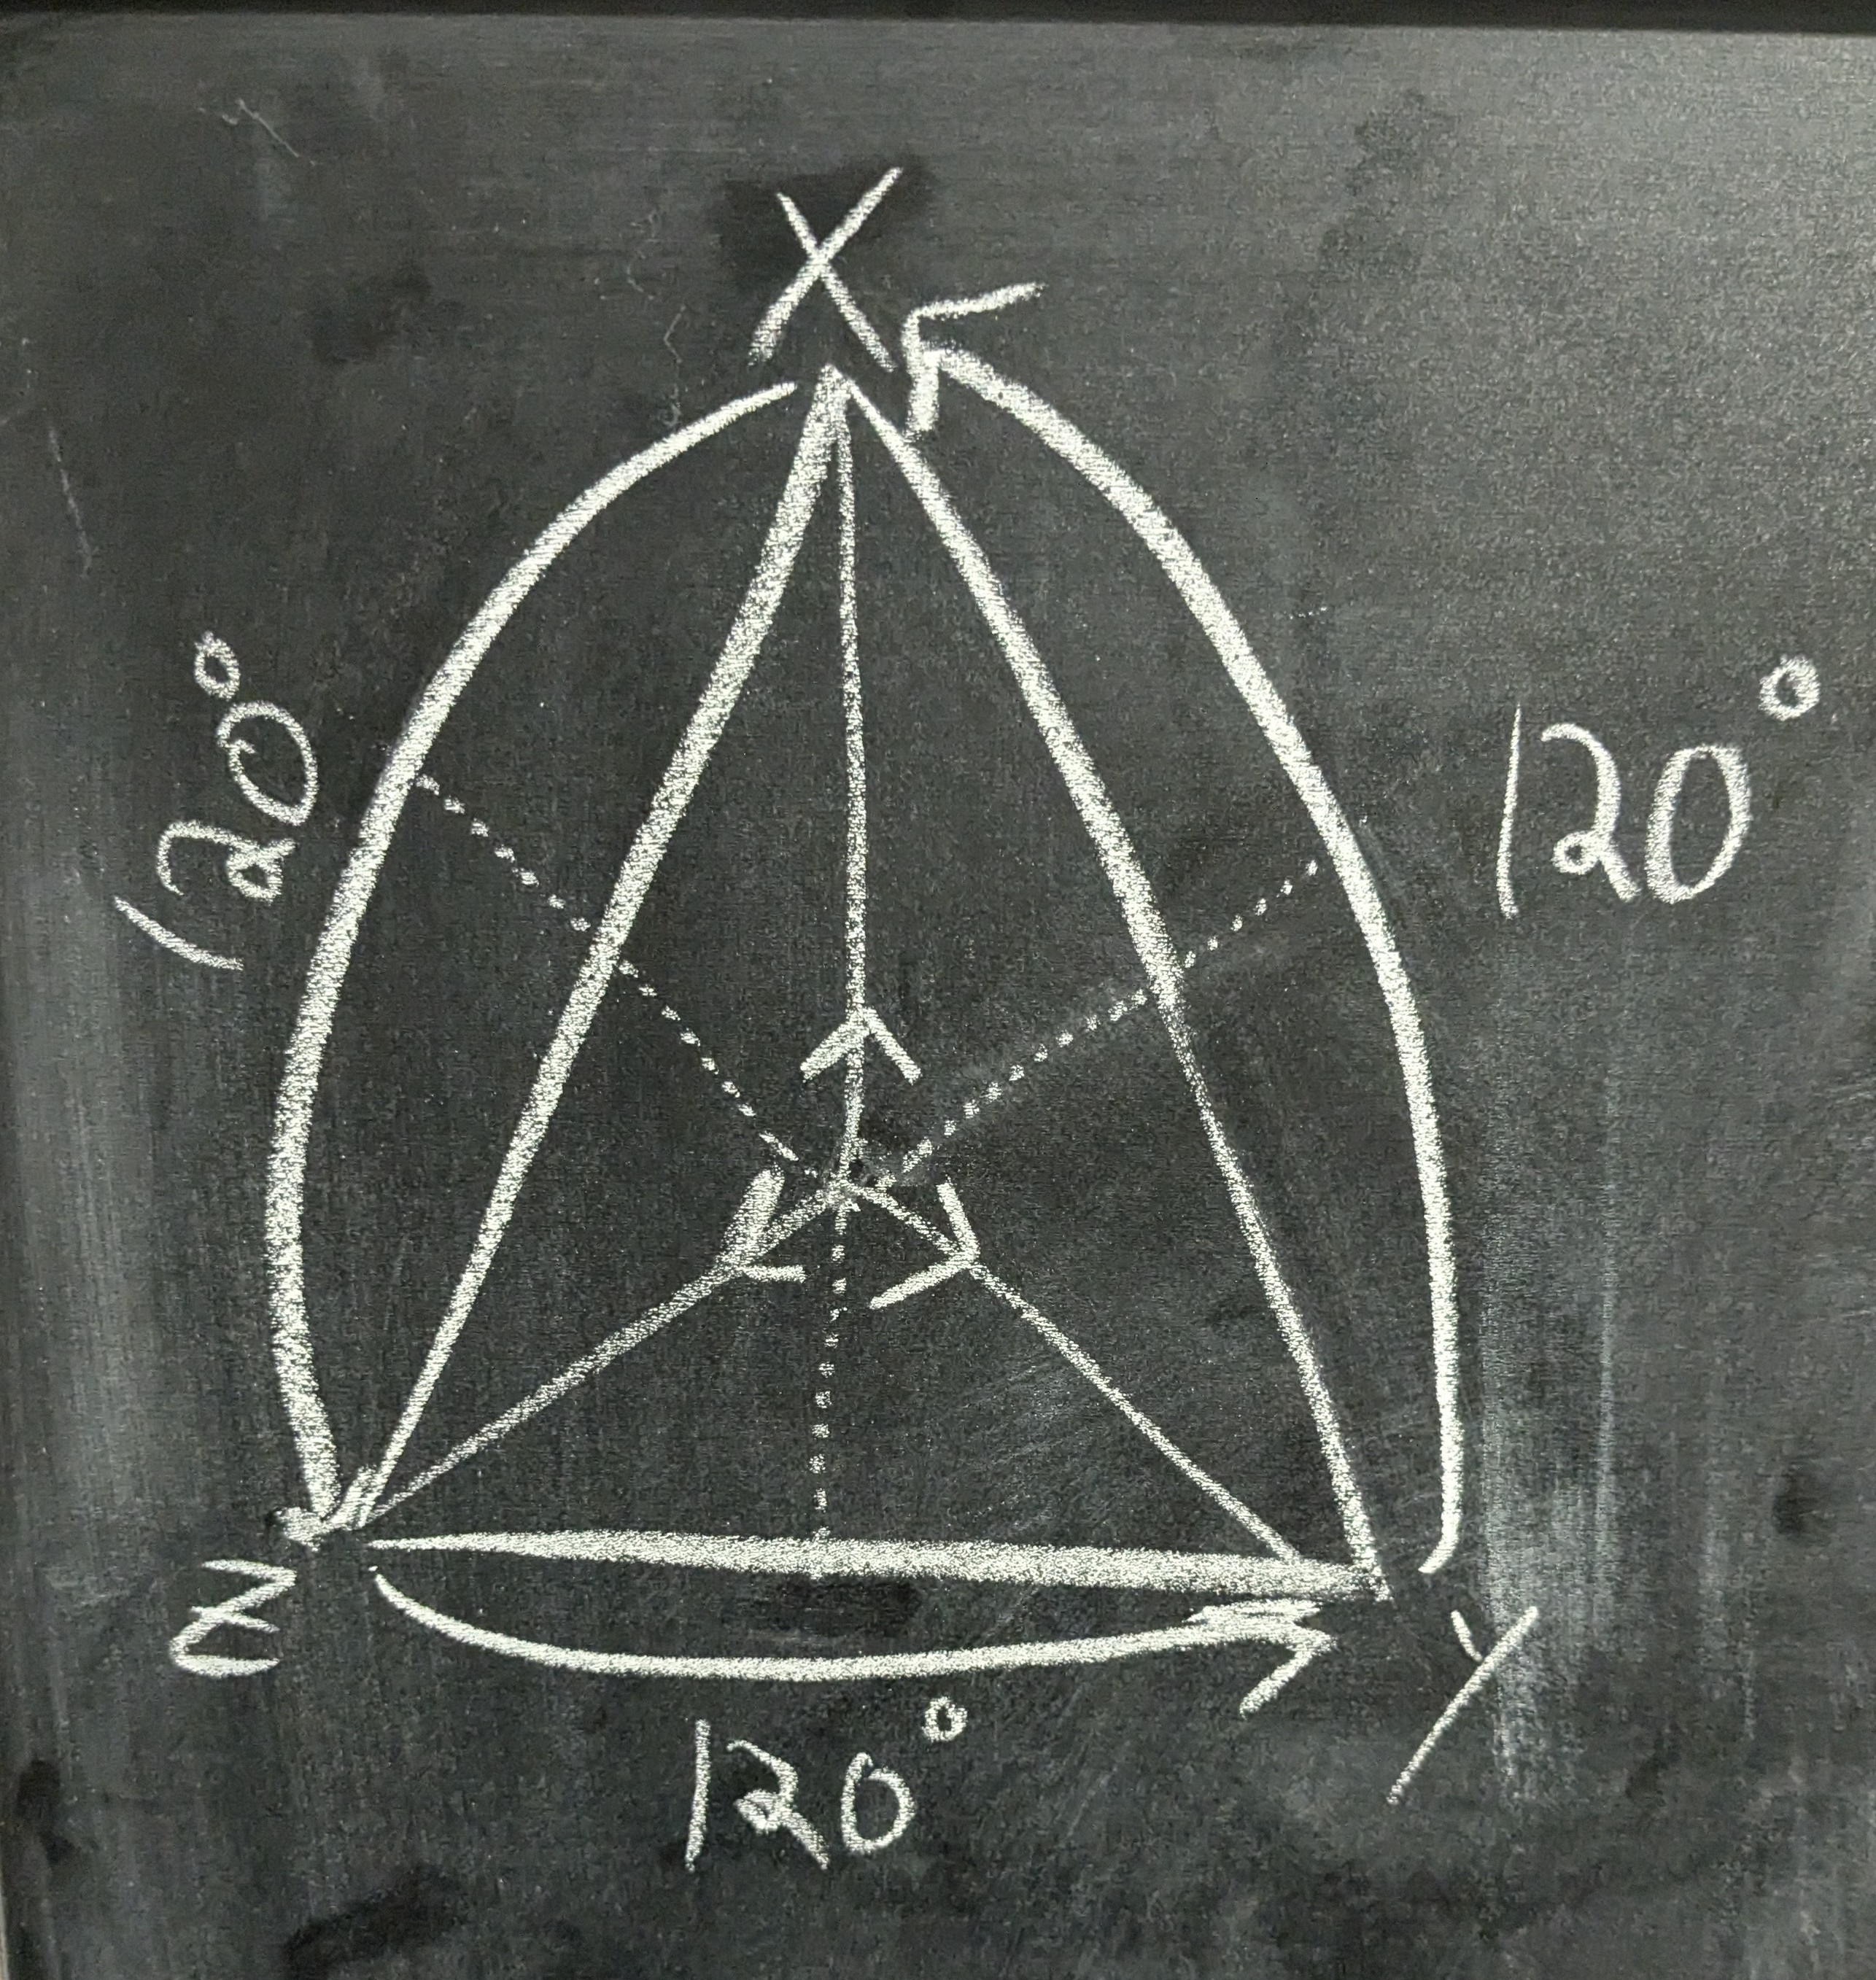
\includegraphics[scale=0.05]{pmechhw1prob1}}

$$
\vec{A} = 
\begin{pmatrix}
    1 & 0 & 0 \\
	0 & 1 & 0  \\
	0 & 0 & 1 \\
\end{pmatrix} \rightarrow
\begin{matrix}
    x & \rightarrow & z \\
	y & \rightarrow & x  \\
	z & \rightarrow & y \\
\end{matrix} \implies \vec{A^{\prime}}
\begin{pmatrix}
    0 & 0 & 1 \\
	1 & 0 & 0  \\
	0 & 1 & 0 \\
\end{pmatrix}
$$

Using $
\lambda_{ij} = Cos(X^{\prime}, X_j)
$
$$
\vec{A^{\prime}} = 
\begin{pmatrix}
    Cos(x^{\prime}, x) & Cos(x^{\prime}, y) & Cos(x^{\prime}, z) \\
	Cos(y^{\prime}, x) & Cos(y^{\prime}, y) & Cos(y^{\prime}, z)  \\
	Cos(z^{\prime}, x) & Cos(z^{\prime}, y) & Cos(z^{\prime}, z) \\
\end{pmatrix} =
\begin{pmatrix}
    Cos(90^{\circ}) & Cos(90^{\circ}) & Cos(0) \\
	Cos(0) & Cos(90^{\circ}) & Cos(90^{\circ})  \\
	Cos(90^{\circ}) & Cos(0) & Cos(90^{\circ}) \\
\end{pmatrix}
$$

$$
\boldsymbol
{
\vec{A^{\prime}} =
\begin{pmatrix}
    0 & 0 & 1 \\
	1 & 0 & 0  \\
	0 & 1 & 0 \\
\end{pmatrix}
}
$$

\newpage
\textbf{(2). Take $\vec{\lambda}$ to be a two-dimensional orthogonal transformation matrix. Show by
direct expansion that $|\vec{\lambda}|^2 = 1$.}

$$
\vec{\lambda} =
\begin{vmatrix}
	\lambda_{11} & \lambda_{12} \\
	\lambda_{21} & \lambda_{22}\\
\end{vmatrix}
= (\lambda_{11}\lambda_{22} - \lambda_{12}\lambda_{21}) \rightarrow \vec{\lambda}^2 = (\lambda_{11}\lambda_{22} - \lambda_{12}\lambda_{21})(\lambda_{11}\lambda_{22} - \lambda_{12}\lambda_{21}) 
$$

$$
\vec{\lambda}^2 = \lambda_{11}^2\lambda_{22}^2 + \lambda_{12}^2\lambda_{21}^2 - 2\lambda_{11}\lambda_{22}\lambda_{12}\lambda_{21}
$$

Using 
$$
\Sigma^{2}_{j} = \lambda_{ij}\lambda_{kj} = \delta_{ik} \rightarrow \lambda_{i1}\lambda_{k1} + \lambda_{i2}\lambda_{k2} = \delta_{ik}
$$

$\mathscr{L}$et i=1,k=1

$$
A = \lambda_{11}\lambda_{11} + \lambda_{12}\lambda_{12} = \delta_{11} = 1
$$

$\mathscr{L}$et i=2,k=2

$$
B = \lambda_{21}\lambda_{21} + \lambda_{22}\lambda_{22} = \delta_{22} = 1
$$

$\mathscr{L}$et i=1,k=2

$$
C = \lambda_{11}\lambda_{21} + \lambda_{12}\lambda_{22} = \delta_{12} = 0 
$$

$\mathscr{L}$et i=2,k=1

$$
D = \lambda_{21}\lambda_{11} + \lambda_{22}\lambda_{12} = \delta_{21} = 0
$$

From A,B,C,D,

$$
AB = (\lambda_{11}^2 + \lambda_{12}^2)(\lambda_{21}^2 + \lambda_{22}^2) = (\lambda_{11}^2\lambda_{21}^2 + \lambda_{11}^2\lambda_{22}^2 + \lambda_{12}^2\lambda_{21}^2 + \lambda_{12}^2\lambda_{22}^2) = 1
$$

$$
CD = (\lambda_{11}\lambda_{21} + \lambda_{12}\lambda_{22})(\lambda_{21}\lambda_{11} + \lambda_{22}\lambda_{12}) = (\lambda_{11}^2\lambda_{21}^2 + \lambda_{12}^2\lambda_{22}^2 + 2\lambda_{11}\lambda_{22}\lambda_{12}\lambda_{21}) = 0 
$$

$$
AB - CD = (\lambda_{11}^2\lambda_{21}^2 + \lambda_{11}^2\lambda_{22}^2 + \lambda_{12}^2\lambda_{21}^2 + \lambda_{12}^2\lambda_{22}^2) - (\lambda_{11}^2\lambda_{21}^2 + \lambda_{12}^2\lambda_{22}^2 + 2\lambda_{11}\lambda_{22}\lambda_{12}\lambda_{21}) = 1 - 0
$$
$$
= \lambda_{11}^2\lambda_{22}^2 + \lambda_{12}^2\lambda_{21}^2 - 2\lambda_{11}\lambda_{22}\lambda_{12}\lambda_{21} = 1
$$

$$\mathbf{AB - CD = |\vec{\lambda}^2| = 1}$$


\newpage
\textbf{(3). Show that $\Sigma_i \lambda_{ij}\lambda_{ik} = \delta_{jk}$ can be obtained by using the requirement that the transformation leaves unchanged the length of a line segment.}

$$
L = \sqrt{\Sigma_i X^2_i}, L^{\prime} = \sqrt{\Sigma_i X^{\prime}^2_i} 
$$

$$
L = L^{\prime} \implies \Sigma_i X^2_i = \Sigma_i X^{\prime}^2_i = X^{\prime}_i = \Sigma_j \lambda_{ij} X_j
$$

$$
\Sigma_i X^2_i = \Sigma_i [(\Sigma_k \lambda_{ik}X_k)(\Sigma_l \lambda_{ik} X_l)] = \Sigma_i X_k X_l (\Sigma_{k,l} \lambda_{ik}\lambda_{il})
$$

\hfill \break

For $\Sigma_i X^2_i = \Sigma_i X_k X_l (\Sigma_{k,l} \lambda_{ik}\lambda_{il})$ to hold true, $\Sigma_{k,l} \lambda_{ik}\lambda_{il} = \delta_{kl}$ 

\hfill \break

Which implies that $\boldsymbol{\Sigma_i \lambda_{ij}\lambda_{ik} = \delta_{jk}}$

\newpage
\textbf{(4). Consider the following matrices:}

$$
\vec{A} = 
\begin{pmatrix}
    1 & 2 & -1 \\
	0 & 3 & 1  \\
	2 & 0 & 1 \\
\end{pmatrix}
,
\vec{B} =
\begin{pmatrix}
    2 & 1 & 0 \\
	0 & -1 & 2\\
	1 & 1 & 3 \\
\end{pmatrix}
,
\vec{C} =
\begin{pmatrix}
    2 & 1 \\
	4 & 3 \\
	1 & 0\\
\end{pmatrix}
$$

\hfill \break

\textbf{Find the following:}
\boldsymbol{

(a): $|\vec{A}\vec{B}|$

(b): $\vec{A}\vec{C}$

(c): $\vec{A}\vec{B}\vec{C}$

(d): $\vec{A}\vec{B} - \vec{A}^T\vec{B}^T$
}

\hfill \break
(a)
$$
\vec{A}\vec{B} = 
\begin{pmatrix}
    1 & 2 & -1 \\
	0 & 3 & 1  \\
	2 & 0 & 1 \\
\end{pmatrix}
\begin{pmatrix}
    2 & 1 & 0 \\
	0 & -1 & 2\\
	1 & 1 & 3 \\
\end{pmatrix} =
\begin{pmatrix}
    2-1 & 1-2-1 & 4-3 \\
	1 & -3+1 & 6+3\\
	4+1 & 2+1 & 3 \\
\end{pmatrix} =
\begin{pmatrix}
    1 & -2 & 1 \\
	1 & -2 & 9\\
	5 & 3 & 3 \\
\end{pmatrix}
$$
$$
\mathbf{|\vec{A}\vec{B}|} = 1(-6-27)-(-2)(3-45) + (3+10) = -33 - 84 + 13 = \boldsymbol{-104}
$$

\hfill \break
(b)
$$
\boldsymbol{\vec{A}\vec{C}} = 
\begin{pmatrix}
    1 & 2 & -1 \\
	0 & 3 & 1  \\
	2 & 0 & 1 \\
\end{pmatrix}
\begin{pmatrix}
    2 & 1 \\
	4 & 3 \\
	1 & 0\\
\end{pmatrix}=
\begin{pmatrix}
    2+8-1 & 1+6 \\
	12+1 & 9 \\
	4+1 & 2\\
\end{pmatrix} =
\boldsymbol{
\begin{pmatrix}
    9 & 7 \\
	13 & 9 \\
	5 & 2\\
\end{pmatrix}
}
$$

\hfill \break
(c)

$$
\boldsymbol{\vec{A}\vec{B}\vec{C}} = (\vec{A}\vec{B})\vec{C} =
\begin{pmatrix}
    1 & 2 & -1 \\
	0 & 3 & 1  \\
	2 & 0 & 1 \\
\end{pmatrix}
\begin{pmatrix}
    2 & 1 & 0 \\
	0 & -1 & 2\\
	1 & 1 & 3 \\
\end{pmatrix}
\begin{pmatrix}
    2 & 1 \\
	4 & 3 \\
	1 & 0\\
\end{pmatrix} = 
\begin{pmatrix}
    1 & -2 & 1 \\
	1 & -2 & 9\\
	5 & 3 & 3 \\
\end{pmatrix}
\begin{pmatrix}
    2 & 1 \\
	4 & 3 \\
	1 & 0\\
\end{pmatrix} = 
\boldsymbol{
\begin{pmatrix}
    -5 & -5 \\
	3 & -5 \\
	25 & 14\\
\end{pmatrix}
}
$$

\hfill \break
(d)

$$
\vec{A}^T = 
\begin{pmatrix}
    1 & 0 & 2 \\
	2 & 3 & 0\\
	-1 & 1 & 1 \\
\end{pmatrix}
,
\vec{B}^T = 
\begin{pmatrix}
    2 & 0 & 1 \\
	1 & -1 & 1\\
	0 & 2 & 3 \\
\end{pmatrix} \rightarrow
\vec{B}^T\vec{A}^T =
\begin{pmatrix}
    2 & 0 & 1 \\
	1 & -1 & 1\\
	0 & 2 & 3 \\
\end{pmatrix}
\begin{pmatrix}
    1 & 0 & 2 \\
	2 & 3 & 0\\
	-1 & 1 & 1 \\
\end{pmatrix} =
\begin{pmatrix}
    1 & 1 & 5 \\
	-2 & -2 & 3\\
	1 & 9 & 3 \\
\end{pmatrix}
$$

$$
\boldsymbol{\vec{A}\vec{B} - \vec{B}^T\vec{A}^T} = 
\begin{pmatrix}
    1 & -2 & 1 \\
	1 & -2 & 9\\
	5 & 3 & 3 \\
\end{pmatrix} -
\begin{pmatrix}
    1 & 1 & 5 \\
	-2 & -2 & 3\\
	1 & 9 & 3 \\
\end{pmatrix} = 
\boldsymbol{
\begin{pmatrix}
    0 & -3 & -4 \\
	3 & 0 & 6\\
	4 & -6 & 0 \\
\end{pmatrix}
}
$$

\newpage
\textbf{(5). Find the value(s) of $\alpha$ needed to make the following transformation matrix
orthogonal.}

$$
\vec{A} = 
\begin{pmatrix}
    1 & 0 & 0 \\
	0 & \alpha & -\alpha\\
	0 & \alpha & \alpha \\
\end{pmatrix} \rightarrow
\vec{A}\vec{A}^T = 
\begin{pmatrix}
    1 & 0 & 0 \\
	0 & \alpha & -\alpha\\
	0 & \alpha & \alpha \\
\end{pmatrix}
\begin{pmatrix}
    1 & 0 & 0 \\
	0 & \alpha & \alpha\\
	0 & -\alpha & \alpha \\
\end{pmatrix} =
\begin{pmatrix}
    1 & 0 & 0 \\
	0 & \alpha^2 + \alpha^2 & \alpha^2 - \alpha^2\\
	0 & \alpha^2 - \alpha^2 & \alpha^2 + \alpha^2 \\
\end{pmatrix}
$$

$$
\vec{A}\vec{A}^T = \vec{I} =
\begin{pmatrix}
    1 & 0 & 0 \\
	0 & \alpha^2 + \alpha^2 & \alpha^2 - \alpha^2\\
	0 & \alpha^2 - \alpha^2 & \alpha^2 + \alpha^2 \\
\end{pmatrix} =
\begin{pmatrix}
    1 & 0 & 0 \\
	0 & 1 & 0\\
	0 & 0 & 1 \\
\end{pmatrix}
$$

$$
\therefore \alpha^2 + \alpha^2 = 1, \alpha^2 - \alpha^2 = 0 \boldsymbol{\alpha = \pm\frac{\sqrt{2}}{2}}
$$

$$
2\alpha^2 = 1 \implies \boldsymbol{\alpha = \pm\frac{\sqrt{2}}{2}}
$$

\end{document}
